%  Formatting the Paper  -------------------------------------------------------
\documentclass[a4paper,11pt]{report}

% adjust margins
\usepackage[right=1in,top=1in,left=1in,bottom=1in]{geometry}


%  Packages Used  --------------------------------------------------------------
\usepackage[english]{babel}
\usepackage[pdftex]{color,graphicx}   % graphics (images)
\usepackage{amsmath}


%  Start the Paper  ------------------------------------------------------------
% define the title
\title{Project 2 - Probabilistic State Estimation Part A}
\author{Qandeel Sajid and Tina Nye}
\begin{document}
\maketitle

% insert the table of contents
\newpage
\tableofcontents
\newpage

\section{Project Description}
Due to the prevalent increase of fraudulent charges from identity theft, the financial industry uses AI algorithms to analyze a card holder's pattern of purchases.  The first part of this assignment implements one of these algorithms: Bayesian Networks.  The Bayesian Network predicts whether a purchase is legitimate by using statistical data on purchase circumstances as random variables with probabilities.  The dependencies for the random variables were predetermined prior to implementing the algorithm and are shown below in the form of a graph. This paper provides and compares the manually computed probabilities for the queries from the project description with those generated by the program.

\section{Implementation}
The program for this project is implemented using Python. The program takes queries provided by the users as well as evidence. The program implements Likelihood Weighting for approximating probabilities. In the algorithm, the variables that are not evidence are sampled and the values for weights are updated using the evidence variables. Weights for a specific event are summed and divided by the summed weights of all events to give the probability for that specific event.


\section{Questions}
	\subsection{Question 1}
	 Figure~\ref{fig:visual} visualizes the information provided in the project description in the form of a Bayesian Network. The nodes are the random variables:

	{\it OC-card holder owns a computer or smart phone.
	
	Fraud-current transaction is fraudulent.
	
	Trav-card holder is currently traveling.
	
	FP-current transaction is a foreign purchase.
	
	IP-current purchase is an internet purchase.
	
	CRP-a computer related purchase was made in the past week.} 

	The arrows in the graph represent dependencies. The Figure also shows the given probabilities for each random variables.
	%show image
	\begin{figure}[h!]
	    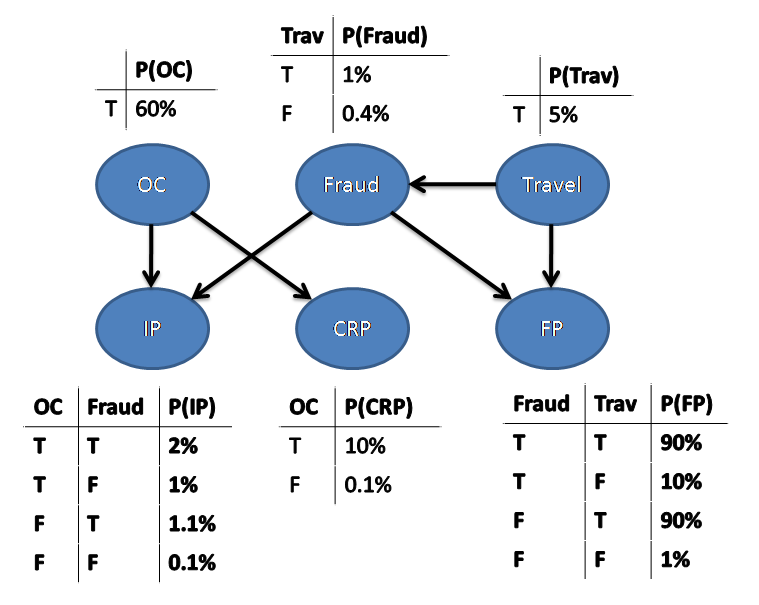
\includegraphics[width=.7\textwidth]{images/partAgraph.png}
	  \caption{Visualization of the Bayesian Network}
	  \label{fig:visual}
	\end{figure}


	\subsection{Question 2}
		\subsubsection{2a - Manual}
			   \begin{align*}
			   &P(Fraud) = \displaystyle\sum\limits_{Trav} P(Fraud|Trav)P(Trav) \\
			   &= P(Fraud|Trav)P(Trav) + P(Fraud|\neg Trav)P(\neg Trav) \\
			   &= 0.01*0.05 + 0.004*0.95 \\
			   &= 0.0043
			   \end{align*}
		   
		 \subsubsection{2a - Inference Algorithm Approximation and Comparisons}
		 	Table 1 shows the output by the Likelihood Weighting algorithm implementation for varying sample sizes. 
		         \begin {table}[h]
			\begin{tabular*}{0.235\textwidth}[left]{|l|l|}
			\hline
			  Samples & \multicolumn{1}{|c|}{P(Fraud)} \\
			  \hline
			  100 & 0.01 \\
			  1000 & 0.006 \\
			  10000 & 0.0052  \\
			  100000 & 0.00418 \\
			  1000000 & 0.004386 \\
			  \hline
			\end{tabular*}
			    \caption{Shows the output P(Fraud) by the program for varying sample values.}
			\end{table}
		
			As shown by the results of the program, the probability of Fraud with 1000000 samples is 1.96 percent different than the manually computed value. The table also shows that as the number of samples increase, the probability calculated by sampling converges with the manually computed solution.
			
		\subsubsection{2b - Manual}
		   \begin{align*}
		   &P(Fraud|FP, \neg IP, CRP) = \frac{P(Fraud \wedge FP \wedge \neg IP \wedge CRP)}{P(FP \wedge \neg IP \wedge CRP)} =\alpha P(Fraud \wedge FP \wedge \neg IP \wedge CRP)\\
		   &\alpha =  \frac{1}{P(FP \wedge \neg IP \wedge CRP)} \\
		   &P(Fraud|FP, \neg IP, CRP) = \\
		   &= \alpha \displaystyle\sum\limits_{Trav} \displaystyle\sum\limits_{OC} P(Fraud|Trav) P(FP|Fraud, Trav) P(\neg IP|Fraud, OC) P(CRP|OC) P(OC) P(Trav) \\
		   &= \alpha(0.004*0.1*0.989*0.001*0.4*0.95 \\
		      &+ 0.004*0.1*0.98*0.1*0.6*0.95 \\
		      &+ 0.01*0.9*0.989*0.001*0.4*0.05 \\
		      &+ 0.01*0.9*0.98*0.1*0.6*0.05) \\
		   &=\alpha 4.913e^{-5}
		   \end{align*}
		
		The value of $\alpha$ can be calculated by finding the probability of $P(\neg Fraud \wedge FP \wedge \neg IP \wedge CRP)$ as the following computations show:
		
		   \begin{align*}
		   &\displaystyle\sum\limits_{Trav} \displaystyle\sum\limits_{OC} P(\neg Fraud|Trav) P(FP| \neg Fraud, Trav) P(\neg IP|OC, \neg Fraud) P(CRP|OG) P(OC) P(Trav) \\
		   &= 0.996*0.01*0.999*0.001*0.4*0.95 \\
		      &+ 0.996*0.01*0.99*0.1*0.6*0.95 \\
		      &+ 0.99*0.9*0.999*0.001*0.4*0.5 \\
		      &+ 0.99*0.9*0.99*0.1*0.6*0.05 \\
		   &= 0.003229
		   \end{align*}
		   
		     \begin{align*}
		   &\alpha = \frac{1}{P(Fraud \wedge FP \wedge \neg IP \wedge CRP) +P(\neg Fraud \wedge FP \wedge \neg IP \wedge CRP)} \\
		   &\alpha = \frac{1}{4.913e^{-5} +  0.003229} \\
		    \end{align*}
		    
		    The $\alpha$ is used to find the $P(Fraud|FP, \neg IP, CRP)$:
		    \begin{align*}
		   &P(Fraud|FP, \neg IP, CRP)= 0.015
		   \end{align*}
		   
		 \subsubsection{2b - Inference Algorithm Approximation and Comparisons}
		 	Table 2 displays the output by the implementation of the Likelihood Weighting algorithm for varying sample sizes. 
		         \begin {table}[h]
			\begin{tabular*}{0.42\textwidth}[left]{|l|l|}
			\hline
			  Samples & \multicolumn{1}{|c|}{$P(Fraud|FP, \neg IP, CRP)$} \\
			  \hline
			  100 & 0.0 \\
			  1000 & 0.0098 \\
			  10000 & 0.0085  \\
			  100000 & 0.0155 \\
			  1000000 & 0.0149 \\
			  \hline
			\end{tabular*}
			    \caption{Shows the output $P(Fraud|FP, \neg IP, CRP)$ by the program for varying sample values.}
			\end{table}
			
			The results of the program show the $P(Fraud|FP, \neg IP, CRP)$ with 1000000 samples is .67 percent different than the manually computed value. The results also show the probability computed by the program converges to the manually computed probability as the number of samples increase.

   \subsection{Question 3}
	For this problem the Trav variable is set to true since we know the owner is traveling and iteration is done over only OC.

	   \begin{align*}
	   &P(Fraud|FP, \neg IP, CRP, Trav) = \\
	   &\alpha \displaystyle\sum\limits_{OC} P(Fraud|Trav) P(FP|Fraud, Trav) P(\neg IP|OC, Fraud) P(CRP|OC) P(OC) P(Trav) \\
	   &=\alpha ( 0.01*0.9*0.98*0.1*0.05*0.6 \\
	      &+ 0.01*0.9*0.989*0.001*0.05*0.4) \\
	   &= \alpha 2.66e^{-5}
	   \end{align*}
	
	   The value of $\alpha$ can be calculated by finding the probability of $P(\neg Fraud \wedge FP \wedge \neg IP \wedge CRP \wedge Trav)$ as the following computations show:
	   \begin{align*}
	   &\displaystyle\sum\limits_{OC} P(\neg Fraud|Trav) P(FP|\neg Fraud, Trav) P(\neg IP|OC, \neg Fraud) P(CRP|OC) P(OC) P(Trav) \\
	   &=( 0.99*0.9*0.99*0.1*0.6*0.05 + 0.94*0.9*0.999*0.001*0.4*0.05) \\
	   &= 0.00266
	   \end{align*}
	
	
	   \begin{align*}
	    &\alpha = \frac{1}{P(Fraud \wedge FP \wedge \neg IP \wedge CRP \wedge Trav) +P(\neg Fraud \wedge FP \wedge \neg IP \wedge CRP \wedge Trav)} \\
	   &\alpha = \frac{1}{2.66e^{-5} + 0.00266} \\
	   &P(Fraud|FP, \neg IP, CRP, Trav) = 0.0099 \\
	   \end{align*}

	Table 3 shows the program's output:
			         \begin {table}[h]
			\begin{tabular*}{0.48\textwidth}[left]{|l|l|}
			\hline
			  Samples & \multicolumn{1}{|c|}{$P(Fraud|FP, \neg IP, CRP, Trav)$} \\
			  \hline
			  100 & 0.0175 \\
			  1000 & 0.0066 \\
			  10000 & 0.0103  \\
			  100000 & 0.0102 \\
			  1000000 & 0.0100 \\
			  \hline
			\end{tabular*}
			    \caption{Shows the output $P(Fraud|FP, \neg IP, CRP, Trav)$ by the program for varying sample values.}
			\end{table}

	\subsection{Question 4}
		   The easiest way to avoid being caught for fraud in the problem is to buy some computer related purchases. The probability of fraud decreases when a thief makes an internet purchase if the fraud detection system believes the card holder owns a computer which can be implied through computer related purchases. 
		   The following probabilities were found using the program:
		   $P(Fraud|IP)=0.0109$
		   
		   $P(Fraud|IP, CRP)=.0084$
		   
		   As shown by the probabilities, the probability of fraud given only internet purchase is higher than the probability of fraud given internet and computer related purchase. By doing a computer related purchase the probability of fraud dropped by 29.76 percent. 



\end{document}
